\chapter{Measuring Mass}\label{ch:g3:measuring-mass}

At the market: ``A \omterm{def:g3:measuring-mass:units}{kilogram} of apples, please!'' The seller pours
apples into the pan until the scale is satisfied. What exactly did
the customer order --- and how does the scale know when to stop?
With \omterm{def:g3:levers-and-scales:lever}{levers} and \omterm{def:g3:levers-and-scales:scale}{balance scales} in our toolbox, we are ready to
\omterm{def:g2:measuring-length:measure}{measure} a new thing: \omterm{def:g3:measuring-mass:mass}{mass}.

\section{Mass: how much stuff}

\begin{definition}[Mass]\label{def:g3:measuring-mass:mass}
The \emph{mass}\index{mass} of a thing tells how much stuff it is
made of. The more stuff, the greater the mass --- and the harder the
Earth pulls it down, which is why things with more mass feel heavier
in your hand and press their pan of a \omterm{def:g3:levers-and-scales:scale}{balance scale} down.
\end{definition}

\begin{example}[Big is not heavy]\label{ex:g3:measuring-mass:bignotcheavy}
A pillow fills your whole arms, yet you carry it easily. A stone
smaller than your fist strains your wrist. The pillow is big but
holds little stuff --- mostly feathers and \omterm{def:g2:air-around-us:air}{air}; the stone is small
but packed with stuff. \omterm{def:g3:measuring-mass:mass}{Mass} is about \emph{how much stuff}, not
about how much room it takes. (These two ideas, and the tricky
dance between them, meet again in the floating-and-sinking story
one day.)
\end{example}

\begin{definition}[Gram and kilogram]\label{def:g3:measuring-mass:units}
\omterm{def:g3:measuring-mass:mass}{Mass} is measured in \emph{grams}\index{gram} (written \unit{g}) and
\emph{kilograms}\index{kilogram} (written \unit{kg}):
\[
\qty{1}{kg} = \qty{1000}{g}.
\]
A paperclip has a \omterm{def:g3:measuring-mass:mass}{mass} of about \qty{1}{g}; an apple about
\qty{150}{g}; a carton of milk about \qty{1}{kg}; you, a few tens
of kilograms. Like the \omterm{def:g2:measuring-length:units}{metre}, these \omterm{def:g2:measuring-length:measure}{units} are the same for everyone
on Earth.
\end{definition}

\section{Weighing with a balance scale}

\begin{method}[Weighing with blocks]\label{met:g3:measuring-mass:weigh}
To \omterm{def:g2:measuring-length:measure}{measure} a melon's \omterm{def:g3:measuring-mass:mass}{mass} with a \omterm{def:g3:levers-and-scales:scale}{balance scale} and a box of marked
metal blocks (\qty{500}{g}, \qty{200}{g}, \qty{100}{g},
\qty{50}{g}, \dots):
\begin{enumerate}
  \item check the empty scale hangs level;
  \item put the melon in one pan;
  \item add blocks to the other pan, biggest useful ones first,
        until the pans hang level;
  \item add up the blocks: their total is the melon's \omterm{def:g3:measuring-mass:mass}{mass}.
\end{enumerate}
If the pans level with a \qty{500}{g}, a \qty{200}{g} and a
\qty{100}{g} block, the melon's \omterm{def:g3:measuring-mass:mass}{mass} is $500 + 200 + 100 =
\qty{800}{g}$.
\end{method}

\begin{omfigure}
\begin{tikzpicture}[scale=0.85]
  \draw[thick] (5.5,0) -- (5.5,2.6);
  \draw[thick] (4.9,0) -- (6.1,0);
  \draw[very thick] (2.5,2.6) -- (8.5,2.6);
  \fill (5.5,2.6) circle (2.4pt);
  \draw[thick] (2.5,2.6) -- (2.2,1.5) (2.5,2.6) -- (2.8,1.5);
  \draw[thick] (1.9,1.5) .. controls (2.5,1.05) .. (3.1,1.5);
  \draw[thick] (8.5,2.6) -- (8.2,1.5) (8.5,2.6) -- (8.8,1.5);
  \draw[thick] (7.9,1.5) .. controls (8.5,1.05) .. (9.1,1.5);
  \draw[thick, fill=omMeth, fill opacity=0.4] (2.5,1.55) circle (0.42);
  \node[font=\footnotesize] at (2.5,1.55) {melon};
  % all three marked blocks, each with its value
  \draw[thick, fill=omExo, fill opacity=0.4] (8.0,1.2) rectangle (8.55,1.7);
  \node[font=\scriptsize] at (8.28,1.45) {$500$};
  \draw[thick, fill=omExo, fill opacity=0.4] (8.6,1.2) rectangle (8.95,1.5);
  \node[font=\scriptsize] at (8.78,1.35) {$200$};
  \draw[thick, fill=omExo, fill opacity=0.4] (8.1,1.7) rectangle (8.35,1.9);
  \node[font=\scriptsize] at (8.22,1.8) {$100$};
  \node[right, font=\footnotesize, align=left] at (9.35,1.7)
    {$500 + 200 + 100$:\\\qty{800}{g} of blocks};
  \node[below, font=\small] at (5.5,-0.3)
    {level pans: the melon's mass equals the blocks' total};
\end{tikzpicture}

{\small Weighing the melon: blocks are added until the pans level;
their sum is the answer.}
\end{omfigure}

\begin{omfigure}
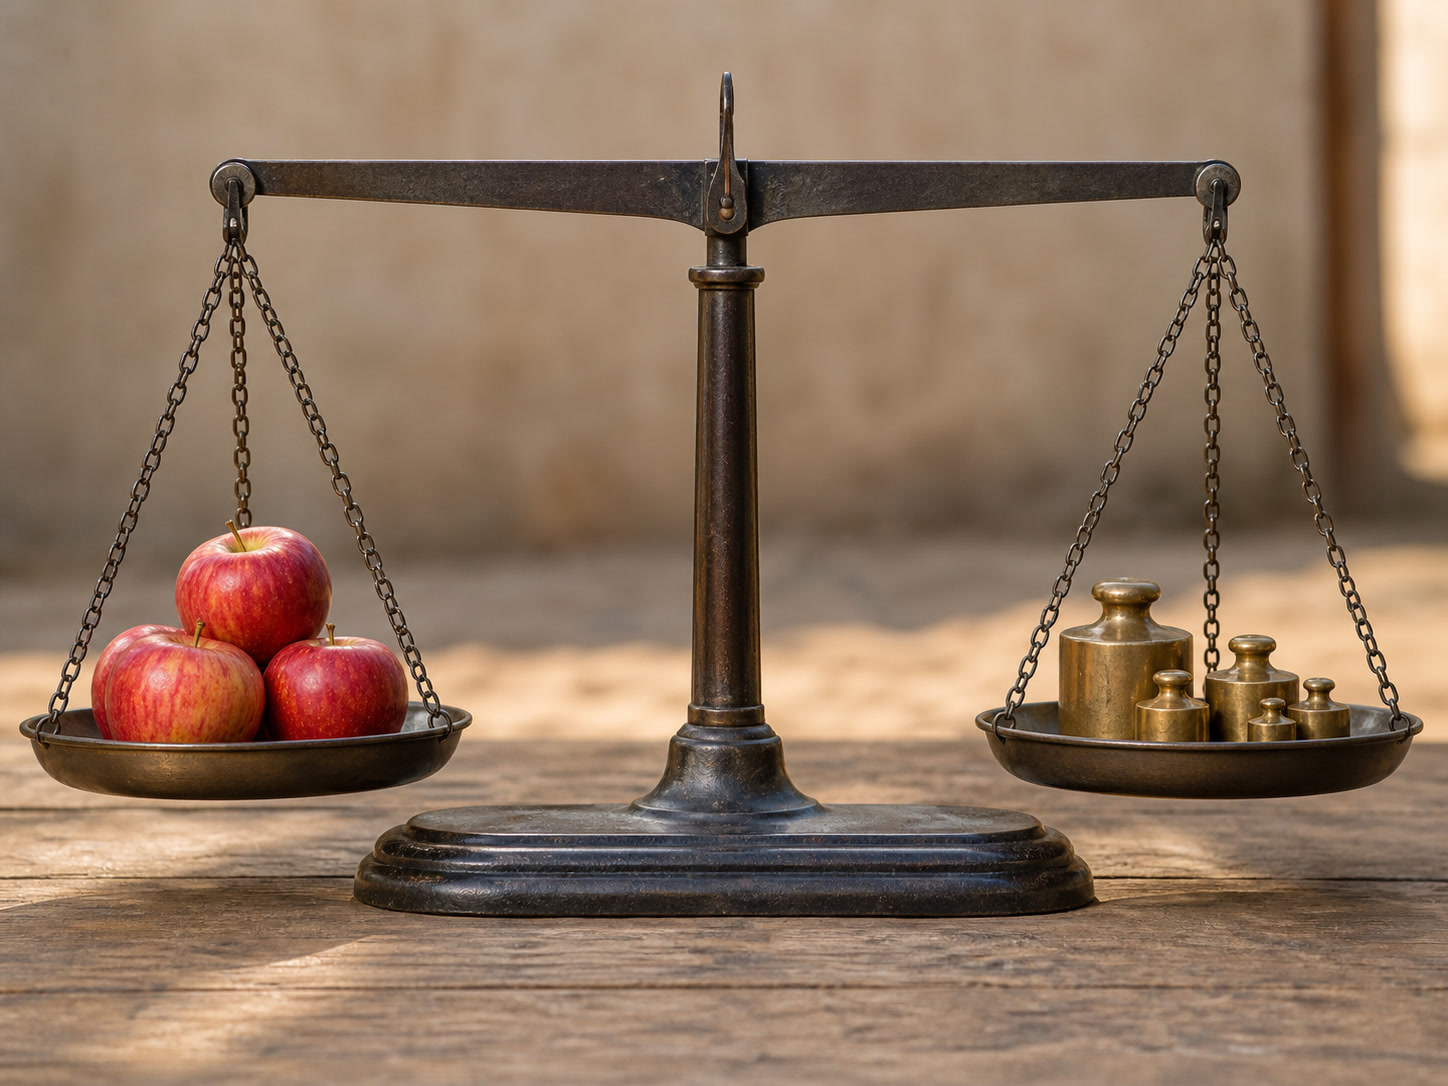
\includegraphics[width=0.52\linewidth]{images/book1/ai/g3-mass-balance-scale.jpg}

{\small A \omterm{def:g3:levers-and-scales:scale}{balance scale} doing its quiet job: level pans, so the apples' \omterm{def:g3:measuring-mass:mass}{mass} equals the brass weights' total.}
\end{omfigure}

\begin{example}[Other scales]\label{ex:g3:measuring-mass:otherscales}
The kitchen scale and the bathroom scale have no second pan: you put
the load on, and a needle turns (or a number \omterm{def:g1:light-and-shadows:source}{lights} up) to show the
\omterm{def:g3:measuring-mass:mass}{mass} directly. Inside, a squeezed spring does the comparing for you.
Handy and fast --- but the old two-pan balance hides no machinery
at all: just the \omterm{def:g3:levers-and-scales:lever}{lever} rule you already understand.
\end{example}

\begin{example}[Reading the market]\label{ex:g3:measuring-mass:market}
``A \omterm{def:g3:measuring-mass:units}{kilogram} of apples'' means: apples until the scale balances a
\qty{1}{kg} block --- about $6$ or $7$ apples. Flour comes in
\qty{1}{kg} bags, chocolate bars are often \qty{100}{g}, a letter
needs about \qty{20}{g} of paper, and the postman's rule ``under
\qty{20}{g}, one stamp'' is a \omterm{def:g3:measuring-mass:mass}{mass} rule.
\end{example}

\section{Mass follows the stuff}

\begin{proposition}[Same stuff, same mass]\label{prop:g3:measuring-mass:conserved}
Changing a thing's \emph{shape} does not change its \omterm{def:g3:measuring-mass:mass}{mass}. Roll a
ball of dough into a snake, flatten it into a pancake, or cut it in
four and weigh all the pieces together: the scale reports the same
\omterm{def:g3:measuring-mass:mass}{mass} every time. \omterm{def:g3:measuring-mass:mass}{Mass} counts the stuff --- and squashing, rolling
and cutting neither add stuff nor take any away.
\end{proposition}

\begin{omfigure}
\begin{tikzpicture}[scale=0.85]
  \draw[thick, omDef!70!black, fill=omDef, fill opacity=0.5]
    (1.3,1.0) circle (0.55);
  \node[below, font=\small, align=center] at (1.3,0.15)
    {a ball of dough:\\\qty{300}{g}};
  \draw[thick, omDef!70!black, fill=omDef, fill opacity=0.5]
    (6.2,0.85) ellipse (1.5 and 0.28);
  \node[below, font=\small, align=center] at (6.2,0.15)
    {rolled into a snake:\\\qty{300}{g}};
  \draw[thick, omDef!70!black, fill=omDef, fill opacity=0.5]
    (9.55,0.75) circle (0.3);
  \draw[thick, omDef!70!black, fill=omDef, fill opacity=0.5]
    (10.28,0.75) circle (0.3);
  \draw[thick, omDef!70!black, fill=omDef, fill opacity=0.5]
    (9.72,1.32) circle (0.28);
  \draw[thick, omDef!70!black, fill=omDef, fill opacity=0.5]
    (10.4,1.32) circle (0.28);
  \node[below, font=\small, align=center] at (10.0,0.15)
    {four pieces together:\\\qty{300}{g}};
\end{tikzpicture}

{\small One lump of dough, three shapes --- and one \omterm{def:g3:measuring-mass:mass}{mass}. The
scale is never fooled by a change of shape.}
\end{omfigure}

\begin{remark}[The scale ignores appearances]\label{rem:g3:measuring-mass:appearances}
This is the quiet power of measuring: eyes judge a flattened pancake
``bigger'' than the ball it came from, and a fluffed pillow
``heavier'' than a stone --- but the \omterm{def:g3:levers-and-scales:scale}{balance scale}, like the
\omterm{def:g3:temperature-thermometers:temperature}{thermometer} and the ruler before it, reports the stuff and nothing
else. One by one, our instruments are replacing ``it seems'' with
``it is''.
\end{remark}

\section{Exercises}

\begin{exercise}[$\star$]\label{exo:g3:measuring-mass:1}
What does the \omterm{def:g3:measuring-mass:mass}{mass} of a thing tell? Which two \omterm{def:g2:measuring-length:measure}{units} \omterm{def:g2:measuring-length:measure}{measure} it, and
how many \omterm{def:g3:measuring-mass:units}{grams} make one \omterm{def:g3:measuring-mass:units}{kilogram}?
\end{exercise}

\begin{exercise}[$\star$]\label{exo:g3:measuring-mass:2}
Choose the likelier \omterm{def:g3:measuring-mass:mass}{mass}: a paperclip --- \qty{1}{g} or \qty{1}{kg}?
An apple --- \qty{150}{g} or \qty{15}{kg}? A carton of milk ---
\qty{1}{g} or \qty{1}{kg}? A cat --- \qty{4}{kg} or \qty{400}{kg}?
\end{exercise}

\begin{exercise}[$\star$]\label{exo:g3:measuring-mass:3}
The pans level when a pumpkin faces a \qty{500}{g} block and two
\qty{200}{g} blocks. What is the pumpkin's \omterm{def:g3:measuring-mass:mass}{mass}?
\end{exercise}

\begin{exercise}[$\star$]\label{exo:g3:measuring-mass:4}
Why must the empty scale hang level before any weighing? (Remember
the cheating merchant.)
\end{exercise}

\begin{exercise}[$\star$]\label{exo:g3:measuring-mass:5}
A beach ball is much bigger than a can of soup, yet the can presses
its pan down. Explain with
\cref{ex:g3:measuring-mass:bignotcheavy}.
\end{exercise}

\begin{exercise}[$\star$]\label{exo:g3:measuring-mass:6}
How many \omterm{def:g3:measuring-mass:units}{grams} are in \qty{2}{kg}? In half a \omterm{def:g3:measuring-mass:units}{kilogram}? Which is
more: \qty{1200}{g} or \qty{1}{kg}?
\end{exercise}

\begin{exercise}[$\star$]\label{exo:g3:measuring-mass:7}
A chocolate bar of \qty{100}{g} is broken into all its little
squares, and every square goes on the scale together. What \omterm{def:g3:measuring-mass:mass}{mass}
does the scale show, and which law says so?
\end{exercise}

\begin{exercise}[$\star$]\label{exo:g3:measuring-mass:8}
The kitchen scale and the two-pan balance both weigh a bag of
flour. What does each use to do the comparing --- and which one
works by a rule you learned three chapters ago?
\end{exercise}

\begin{exercise}[$\star$]\label{exo:g3:measuring-mass:9}
The baker needs \qty{800}{g} of flour and has blocks of
\qty{500}{g}, \qty{200}{g}, \qty{200}{g}, \qty{100}{g} and
\qty{50}{g}. Find two different ways to weigh out exactly
\qty{800}{g} --- knowing that blocks are allowed to sit in
\emph{either} pan.
\end{exercise}

\begin{exercise}[$\star\star$]\label{exo:g3:measuring-mass:10}
Nina weighs a whole orange: \qty{200}{g}. She peels it and weighs
the peeled orange alone: \qty{160}{g}. Has
\cref{prop:g3:measuring-mass:conserved} failed? Where are the
missing \omterm{def:g3:measuring-mass:units}{grams}, and how could Nina prove it with one more weighing?
\end{exercise}

\begin{exercise}[$\star\star$]\label{exo:g3:measuring-mass:11}
A riddle, at last easy for you: which has more \omterm{def:g3:measuring-mass:mass}{mass}, a \omterm{def:g3:measuring-mass:units}{kilogram} of
feathers or a \omterm{def:g3:measuring-mass:units}{kilogram} of iron? And which takes more room? Explain
why so many people answer the first question wrongly.
\end{exercise}
